\documentclass{standalone}
\usepackage{tikz}
\usetikzlibrary{patterns, positioning}
\usepackage[sfdefault]{ClearSans} %% option 'sfdefault' activates Clear Sans as the default text font
\usepackage[T1]{fontenc}

\begin{document}
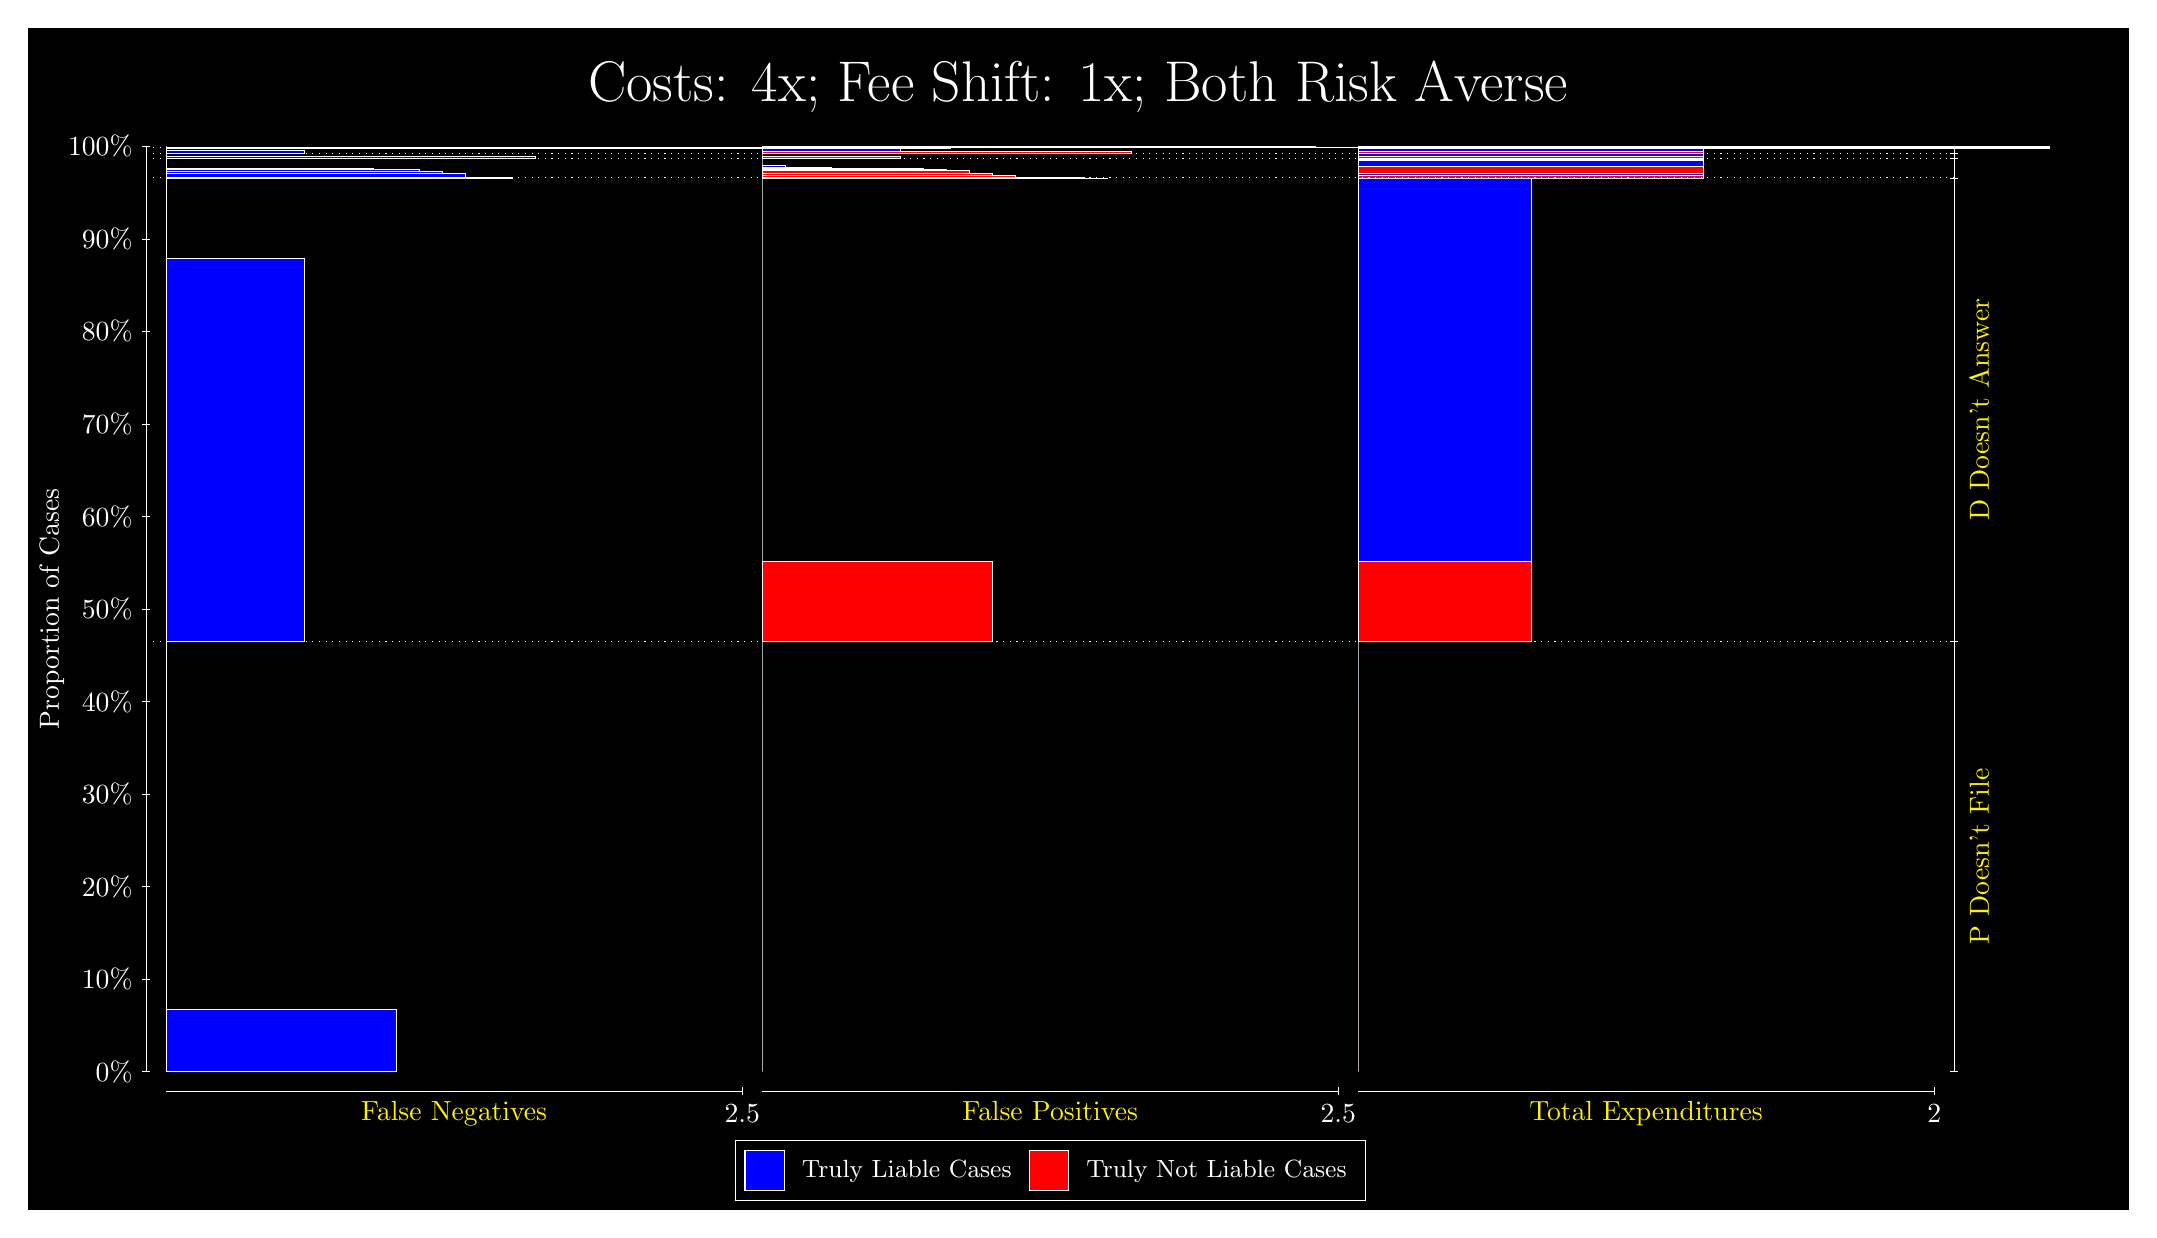
\begin{tikzpicture}
\draw[fill=black] (0,0) rectangle (26.667,15);
\draw[text=white] (0,13.5) rectangle (26.667,15) node[midway] {\huge Costs: 4x; Fee Shift: 1x; Both Risk Averse};
\draw[white, very thin] (1.5,1.75) -- (1.5,13.5);
\node[rotate=90, text=white, anchor=center] at (0.3, 7.625) {Proportion of Cases};
\draw[white, very thin] (1.45,1.75) -- (1.55,1.75);
\node[text=white, anchor=east] at (1.45, 1.75) {0\%};
\draw[white, very thin] (1.45,2.925) -- (1.55,2.925);
\node[text=white, anchor=east] at (1.45, 2.925) {10\%};
\draw[white, very thin] (1.45,4.1) -- (1.55,4.1);
\node[text=white, anchor=east] at (1.45, 4.1) {20\%};
\draw[white, very thin] (1.45,5.275) -- (1.55,5.275);
\node[text=white, anchor=east] at (1.45, 5.275) {30\%};
\draw[white, very thin] (1.45,6.45) -- (1.55,6.45);
\node[text=white, anchor=east] at (1.45, 6.45) {40\%};
\draw[white, very thin] (1.45,7.625) -- (1.55,7.625);
\node[text=white, anchor=east] at (1.45, 7.625) {50\%};
\draw[white, very thin] (1.45,8.8) -- (1.55,8.8);
\node[text=white, anchor=east] at (1.45, 8.8) {60\%};
\draw[white, very thin] (1.45,9.975) -- (1.55,9.975);
\node[text=white, anchor=east] at (1.45, 9.975) {70\%};
\draw[white, very thin] (1.45,11.15) -- (1.55,11.15);
\node[text=white, anchor=east] at (1.45, 11.15) {80\%};
\draw[white, very thin] (1.45,12.325) -- (1.55,12.325);
\node[text=white, anchor=east] at (1.45, 12.325) {90\%};
\draw[white, very thin] (1.45,13.5) -- (1.55,13.5);
\node[text=white, anchor=east] at (1.45, 13.5) {100\%};

\draw[white, very thin] (24.457,1.75) -- (24.457,13.5);
\draw[white, very thin] (24.407,1.75) -- (24.507,1.75);
\node[anchor=west] at (24.407, 1.75) {};
\draw[white, very thin] (24.407,7.2104) -- (24.507,7.2104);
\node[anchor=west] at (24.407, 7.2104) {};
\draw[white, very thin] (24.407,13.099) -- (24.507,13.099);
\node[anchor=west] at (24.407, 13.099) {};
\draw[white, very thin] (24.407,13.342) -- (24.507,13.342);
\node[anchor=west] at (24.407, 13.342) {};
\draw[white, very thin] (24.407,13.408) -- (24.507,13.408);
\node[anchor=west] at (24.407, 13.408) {};
\draw[white, very thin] (24.407,13.48) -- (24.507,13.48);
\node[anchor=west] at (24.407, 13.48) {};
\draw[white, very thin] (24.407,13.488) -- (24.507,13.488);
\node[anchor=west] at (24.407, 13.488) {};
\draw[white, very thin] (24.407,13.5) -- (24.507,13.5);
\node[anchor=west] at (24.407, 13.5) {};

\draw[white, very thin, fill=blue] (1.75,1.75) rectangle (4.6775,2.5437);
\draw[white, very thin, fill=red] (1.75,2.5437) rectangle (1.75,7.2104);
\draw[white, very thin, fill=blue] (1.75,7.2104) rectangle (3.5065,12.083);
\draw[white, very thin, fill=red] (1.75,12.083) rectangle (1.75,13.099);
\draw[white, very thin, fill=blue] (1.75,13.099) rectangle (6.1413,13.103);
\draw[white, very thin, fill=blue] (1.75,13.103) rectangle (5.8486,13.113);
\draw[white, very thin, fill=blue] (1.75,13.113) rectangle (5.5558,13.154);
\draw[white, very thin, fill=blue] (1.75,13.154) rectangle (5.2631,13.177);
\draw[white, very thin, fill=blue] (1.75,13.177) rectangle (4.9703,13.205);
\draw[white, very thin, fill=blue] (1.75,13.205) rectangle (4.6775,13.213);
\draw[white, very thin, fill=blue] (1.75,13.213) rectangle (4.3848,13.22);
\draw[white, very thin, fill=blue] (1.75,13.22) rectangle (4.092,13.222);
\draw[white, very thin, fill=blue] (1.75,13.222) rectangle (3.7993,13.224);
\draw[white, very thin, fill=red] (1.75,13.224) rectangle (1.75,13.342);
\draw[white, very thin, fill=blue] (1.75,13.342) rectangle (6.4341,13.373);
\draw[white, very thin, fill=red] (1.75,13.373) rectangle (1.75,13.408);
\draw[white, very thin, fill=blue] (1.75,13.408) rectangle (3.5065,13.451);
\draw[white, very thin, fill=red] (1.75,13.451) rectangle (1.75,13.48);
\draw[white, very thin, fill=blue] (1.75,13.48) rectangle (11.704,13.482);
\draw[white, very thin, fill=red] (1.75,13.482) rectangle (1.75,13.488);
\draw[white, very thin, fill=red] (1.75,13.488) rectangle (1.75,13.491);
\draw[white, very thin, fill=blue] (1.75,13.491) rectangle (1.75,13.5);
\draw[white, very thin, fill=red] (9.3189,1.75) rectangle (9.3189,6.4168);
\draw[white, very thin, fill=blue] (9.3189,6.4168) rectangle (9.3189,7.2104);
\draw[white, very thin, fill=red] (9.3189,7.2104) rectangle (12.246,8.2272);
\draw[white, very thin, fill=blue] (9.3189,8.2272) rectangle (9.3189,13.099);
\draw[white, very thin, fill=red] (9.3189,13.099) rectangle (13.71,13.1);
\draw[white, very thin, fill=red] (9.3189,13.1) rectangle (13.417,13.101);
\draw[white, very thin, fill=red] (9.3189,13.101) rectangle (13.125,13.105);
\draw[white, very thin, fill=red] (9.3189,13.105) rectangle (12.832,13.112);
\draw[white, very thin, fill=red] (9.3189,13.112) rectangle (12.539,13.138);
\draw[white, very thin, fill=red] (9.3189,13.138) rectangle (12.246,13.161);
\draw[white, very thin, fill=red] (9.3189,13.161) rectangle (11.954,13.201);
\draw[white, very thin, fill=red] (9.3189,13.201) rectangle (11.661,13.212);
\draw[white, very thin, fill=red] (9.3189,13.212) rectangle (11.368,13.218);
\draw[white, very thin, fill=blue] (9.3189,13.218) rectangle (10.783,13.22);
\draw[white, very thin, fill=blue] (9.3189,13.22) rectangle (10.49,13.222);
\draw[white, very thin, fill=blue] (9.3189,13.222) rectangle (10.197,13.229);
\draw[white, very thin, fill=blue] (9.3189,13.229) rectangle (9.9044,13.237);
\draw[white, very thin, fill=blue] (9.3189,13.237) rectangle (9.6116,13.265);
\draw[white, very thin, fill=blue] (9.3189,13.265) rectangle (9.3189,13.342);
\draw[white, very thin, fill=red] (9.3189,13.342) rectangle (11.075,13.377);
\draw[white, very thin, fill=blue] (9.3189,13.377) rectangle (9.3189,13.408);
\draw[white, very thin, fill=red] (9.3189,13.408) rectangle (14.003,13.438);
\draw[white, very thin, fill=blue] (9.3189,13.438) rectangle (11.075,13.48);
\draw[white, very thin, fill=red] (9.3189,13.48) rectangle (9.3189,13.486);
\draw[white, very thin, fill=blue] (9.3189,13.486) rectangle (9.3189,13.488);
\draw[white, very thin, fill=red] (9.3189,13.488) rectangle (19.273,13.491);
\draw[white, very thin, fill=blue] (9.3189,13.491) rectangle (16.345,13.5);
\draw[white, very thin, fill=red] (16.888,1.75) rectangle (16.888,6.4168);
\draw[white, very thin, fill=blue] (16.888,6.4168) rectangle (16.888,7.2104);
\draw[white, very thin, fill=red] (16.888,7.2104) rectangle (19.083,8.2272);
\draw[white, very thin, fill=blue] (16.888,8.2272) rectangle (19.083,13.099);
\draw[white, very thin, fill=red] (16.888,13.099) rectangle (21.279,13.126);
\draw[white, very thin, fill=blue] (16.888,13.126) rectangle (21.279,13.154);
\draw[white, very thin, fill=red] (16.888,13.154) rectangle (21.279,13.241);
\draw[white, very thin, fill=blue] (16.888,13.241) rectangle (21.279,13.329);
\draw[white, very thin, fill=red] (16.888,13.329) rectangle (21.279,13.334);
\draw[white, very thin, fill=blue] (16.888,13.334) rectangle (21.279,13.342);
\draw[white, very thin, fill=red] (16.888,13.342) rectangle (21.279,13.377);
\draw[white, very thin, fill=blue] (16.888,13.377) rectangle (21.279,13.408);
\draw[white, very thin, fill=red] (16.888,13.408) rectangle (21.279,13.438);
\draw[white, very thin, fill=blue] (16.888,13.438) rectangle (21.279,13.48);
\draw[white, very thin, fill=red] (16.888,13.48) rectangle (25.67,13.486);
\draw[white, very thin, fill=blue] (16.888,13.486) rectangle (25.67,13.488);
\draw[white, very thin, fill=red] (16.888,13.488) rectangle (25.67,13.491);
\draw[white, very thin, fill=blue] (16.888,13.491) rectangle (25.67,13.5);
\draw[white, dotted] (1.5,7.2104) -- (24.457,7.2104);
\draw[white, dotted] (1.5,13.099) -- (24.457,13.099);
\draw[white, dotted] (1.5,13.342) -- (24.457,13.342);
\draw[white, dotted] (1.5,13.408) -- (24.457,13.408);
\draw[white, dotted] (1.5,13.48) -- (24.457,13.48);
\draw[white, dotted] (1.5,13.488) -- (24.457,13.488);
\draw[white, very thin] (1.75,1.5) -- (9.0689,1.5);
\node[text=yellow, anchor=north] at (5.4094, 1.5) {False Negatives};
\draw[white, very thin] (9.0689,1.45) -- (9.0689,1.55);
\node[text=white, anchor=north] at (9.0689, 1.45) {2.5};

\draw[white, very thin] (9.3189,1.5) -- (16.638,1.5);
\node[text=yellow, anchor=north] at (12.978, 1.5) {False Positives};
\draw[white, very thin] (16.638,1.45) -- (16.638,1.55);
\node[text=white, anchor=north] at (16.638, 1.45) {2.5};

\draw[white, very thin] (16.888,1.5) -- (24.207,1.5);
\node[text=yellow, anchor=north] at (20.547, 1.5) {Total Expenditures};
\draw[white, very thin] (24.207,1.45) -- (24.207,1.55);
\node[text=white, anchor=north] at (24.207, 1.45) {2};

\node[text=yellow, centered, rotate=90] at (24.777, 4.4802) {P Doesn't File};
\node[text=yellow, centered, rotate=90] at (24.777, 10.155) {D Doesn't Answer};






\draw (12.978300999999998,1.5) node[draw=none] (baseCoordinate) {};
\begin{scope}[align=center]
        \matrix[scale=0.5, draw=white, below=0.5cm of baseCoordinate, nodes={draw}, column sep=0.1cm]{
            \node[rectangle, draw, minimum width=0.5cm, minimum height=0.5cm, fill=blue] {}; &
            \node[draw=none, font=\small, text=white] (B) {Truly Liable Cases}; &
            \node[rectangle, draw, minimum width=0.5cm, minimum height=0.5cm, fill=red] {}; &
            \node[draw=none, font=\small, text=white] (B) {Truly Not Liable Cases}; \\
            };
\end{scope}

\end{tikzpicture}
\end{document}